\begin{filecontents*}{prace.xmpdata}	
	\Title{\druhCZ\ -\ \nazevCZ}
	\Author{\autor}
	\Keywords{\klicovaCZ}
	\Publisher{\skolaCZ}
	\Language{Čeština}
\end{filecontents*}	% Metadata pro PDF/A

\documentclass[a4paper,oneside,12pt,pdftex,czech] {book}
\usepackage{cmap}
\usepackage[utf8]{inputenc}		% kódování textu
\usepackage[T1]{fontenc}		% T1 font
\usepackage{lmodern}			% Latin modern font
\usepackage[main=czech,english]{babel}	% česká tipografie hlavní, anglická jako druhá
\usepackage{lipsum}				% text na vyplnění
\usepackage{blindtext}			% text na vyplnění
\usepackage{fancyhdr}			% uživatelsky definované záhlaví a zápatí
\usepackage{geometry}			% rozměry stránky
\geometry{
	a4paper,					% formát stránky
	includeheadfoot,			% obsažení záhlaví a zápatí do rozměru textu	
	bindingoffset=1cm,			% místo pro vazbu
	left=2.5cm,					% odsazení vlevo
	right=2.5cm,				% odsazení vpravo
	top=0cm,					% odsazení nahoře
	bottom=1cm,					% odsazeni dole
	headheight=2cm,				% výška hlavičky
	footskip=1.5cm,				% mezery mezi textem a zapatim
	headsep=0.5cm}				% mezery mezi zahlavim a textem
\usepackage{pdfpages}			% pdf include
\usepackage{multirow}			% multirow tabulky
\usepackage[titles]{tocloft}	% toc specifikace
\usepackage{siunitx}			% jednotky
\sisetup{
	output-decimal-marker = {,},					% oddělovač desetiných čísel
	output-complex-root = \text{\ensuremath{i}},	% imaginární jednotka
	range-units = brackets,							% rozsah čísel v závorce poté až jednotky
	list-units = brackets,							% seznam čísel v závorce poté až jednotky
	list-final-separator = {~a~},					% poslední a předposlední člen listu je oddělen a
	list-pair-separator = {~a~},					% poslední a předposlední člen listu je oddělen a
	list-separator = {; },							% oddělovač prvků v seznamu
	range-phrase ={~až~},							% rozsah čísel
	inter-unit-product=\ensuremath{{\cdot}},		% uzké mezery u jednotek a vzdy bude tecka
	tight-spacing=true,
}
\usepackage{booktabs}			% orámování tabulek
\usepackage{xltabular}			% dlouhé tabulky a tabulky definové šířky
\usepackage[normalem]{ulem}		% přešktrnutý text
\usepackage{amsmath}			% matematika
\usepackage{amsfonts}			% matematický font
\usepackage{amssymb}			% matematické symboly
\usepackage{mathtools}			% ještě lepší matematika
\usepackage{cases}				% pro funkce definované možnostmi (vidličkou)
\usepackage{xspace}				% přidání mezery na konec makra 
\usepackage{ragged2e}

\setlength{\jot}{2ex} 			% mezery mezi řádky v režimu víceřádkových rovnic

\definecolor{BarvaOdkaz}{RGB}{255, 0, 0}
\definecolor{BarvaURLOdkaz}{RGB}{0, 0, 255}
\definecolor{BarvaLiteratura}{RGB}{0, 255, 0}

\usepackage{relsize}			% různá velikost v matematickém módu
\usepackage[bottom]{footmisc}	% footnote nejníže nastránce
\usepackage{footnotebackref}	% odkaz do textu z poznámky pod čarou
\usepackage[all]{xy}			% diagramy a grafy
\usepackage{wasysym}			% symobly npř. průměr
\usepackage{smartdiagram}		% jednoduchý generátor diagramů
\usepackage{csquotes}			% uvozovky
\usepackage[version=4]{mhchem}	% chemické rovnice
\usepackage{physics}			% fyzika, dobre zejmena pro psani diferencialu
\usepackage[Euler]{upgreek}		% alfabeta bez italiky v rovnicich
\usepackage[euler]{textgreek}	% alfabeta bez italiky v textu
\usepackage[
	backend=biber,				% literatura zpracovávaná bibre
	style=numeric,				% číslování odkazů
	sortcites=true,				% řazení čísel citací v závorkách v textu
	defernumbers=true,			% zachování číslování při použití sekcí v Literaruře
]{biblatex}						% reference 
\usepackage{float}
\usepackage{enumitem}
\usepackage{xcolor, soul} %změna barvy textu a jeho zvýraznění \hl{zvýrazněný text}

\DeclareFieldFormat[online]{urldate}{\mkbibbrackets{\bibstring{urlseen}\space{#1}}}		% zobrazit citováno v závorkách
\DeclareFieldFormat[article]{title}{#1} 										% název článku bez uvozovek
\DeclareFieldFormat[article]{volume}{\mkbibbold{#1}} 							% vydání článku silně
\DeclareFieldFormat[article]{number}{\mkbibparens{#1}}							% číslo článku v závorce
\DeclareFieldFormat[article,online,misc]{note}{\mkbibbrackets{#1}}				% poznámka v hranaté závorce
\DeclareFieldFormat[article,online,misc]{url}{Dostupné~z:\space\url{#1}}		% článek a online místo URL dostupné z:

\addbibresource{mybib.bib}					% dokument literatury

\renewbibmacro*{journal+issuetitle}{%		%  místo vydání a nakladatel v článku
	\usebibmacro{journal}%
	\setunit*{\addperiod\space}%
	\usebibmacro{publisher+location+date}%
	\setunit*{\addcomma\space}%
	\iffieldundef{series}%
	{}
	{\newunit%
		\printfield{series}%
		\setunit{\addcomma\space}}%
	\usebibmacro{volume+number+eid}%
	\setunit{\addspace}%
	\usebibmacro{issue}%
	\newunit}%

\renewbibmacro*{volume+number+eid}{%	% vložení čísla článku tlustě a vydání do závorky a k sobě
	\printfield{volume}%
	\printfield{number}%
	\setunit{\addcomma\space}%
	\printfield{eid}}%

\defbibfilter{zbytek}{	% filtr pro pro ostaní články v online sekci
	type=online or
	type=misc
}

\usepackage{import}	% import z jiné než kořenové složky
\usepackage[final,numbered,framed]{matlab-prettifier}	% pro zdrojový kód Matlabu
\lstset{
	style=Matlab-editor,		% styl kódu Matlab
	basicstyle=\mlttfamily,		% nepatkový font
	escapechar=",				% znak pro Latex ve verbatim prostředí
	xleftmargin=3.4pt,	% odsazení kódu zleva
	xrightmargin=3.4pt,	% odsazení kódu zprava
	captionpos=b,				% popisek umístěn pod kódem
	numberstyle=\color{black},	% barva čísel řádků
	tabsize=4, 					% tab space width
	numbers=right,				% číslování vlevo
	postbreak={\RIGHTarrow},	% znak zalomení řádky
	prebreak={},	
	aboveskip=20pt,
	belowskip=20pt,
	literate={é}{{\'e}}1		% diakritika v komentech
			{č}{{\v{c}}}1
			{Č}{{\v{C}}}1
			{ť}{{\v{t}}}1
			{Ť}{{\v{T}}}1
			{ý}{{\'y}}1
			{ě}{{\v{e}}}1
			{ř}{{\v{r}}}1
			{Ř}{{\v{R}}}1
			{š}{{\v{s}}}1
			{Š}{{\v{S}}}1
			{ž}{{\v{z}}}1
			{Ž}{{\v{Z}}}1
			{á}{{\'a}}1
			{í}{{\'i}}1
			{ó}{{\'o}}1
			{ň}{{\v{n}}}1
			{Ň}{{\v{N}}}1
			{ď}{{\v{d}}}1
			{ú}{{\'u}}1
			{ů}{{\r{u}}}1
			{Ú}{{\'U}}1
			{Ů}{{\r{U}}}1			
}


\usepackage[nameinlink]{cleveref}	% chytré odkazy s překladem do češtiny
\crefname{equation}{rovnice}{rovnice}
\crefname{figure}{obrázek}{obrázky}
\crefname{subfigure}{podobrázek}{podobrázky}
\crefname{table}{tabulka}{tabulky}
\crefname{subtable}{podtabulka}{podtabulky}
\crefname{page}{strana}{strany}
\crefname{part}{část}{části}
\crefname{chapter}{kapitola}{kapitoly}
\crefname{section}{sekce}{sekce}
\crefname{subsection}{podsekce}{podsekce}
\crefname{appendix}{příloha}{přílohy}
\crefname{subappendix}{podpříloha}{podpřílohy}
\crefname{enumi}{bod}{body}%
\crefname{enumii}{bod}{body}%
\crefname{enumiii}{bod}{body}%
\crefname{enumiv}{bod}{body}%%
\crefname{enumv}{bod}{body}%
\crefname{footnote}{poznámka pod čarou}{poznámky pod čarou}%
\crefname{theorem}{teorém}{teorémy}%
\crefname{lemma}{lema}{lama}%
\crefname{corollary}{důsledek}{důsledky}%
\crefname{definition}{definice}{definice}%
\crefname{result}{výsledek}{výsledky}
\crefname{example}{příklad}{příklady}%
\crefname{note}{poznámka}{poznámky}%
\crefname{algorithm}{algoritmus}{algoritmy}%
\crefname{line}{řádka}{řádky}%
\crefname{listing}{algoritmus}{algoritmy}  
\newcommand{\crefrangeconjunction}{ až~}%
\newcommand{\crefpairconjunction}{ a~}%
\newcommand{\crefmiddleconjunction}{, }%
\newcommand{\creflastconjunction}{ a~}%
\newcommand{\crefpairgroupconjunction}{ a~}%
\newcommand{\crefmiddlegroupconjunction}{, }%
\newcommand{\creflastgroupconjunction}{, a~}%

\DeclareNameAlias{author}{family-given} 			% zobrazení v literatuře nejdříve příjmení 
\renewcommand*{\mkbibnamefamily}[1]{\textsc{#1}}	% příjmení autora kapitálkami
\renewcommand{\subtitlepunct}{\addcolon\addspace}	% odelení názvu a podnázvu dvojtečkou v seznamu Literatury
\renewcommand*{\finentrypunct}{}					% odstranění poslední tečky v citaci

\usepackage[]{caption}			% titulky obrázky, tabulky...
\captionsetup{
justification=justified,		% zarovnání titulku na šířku textu 
singlelinecheck=false,			% i jednořádkový popisek stále zarovná do leva
labelfont=bf,					% název popisku tučně
}

\usepackage[justification=justified,singlelinecheck=true]{subcaption}	% podnadpisky zarovnane do bloku, jednořádkový zarovnaný na střed

\setcounter{secnumdepth}{3}	% číslování až do subsubsection
\setcounter{tocdepth}{3}	% zobrazení subsubsection v ToC

\fancyhf{} 																	% vymazání zapati záhlaví
\renewcommand{\headrulewidth}{0pt}											% žádná horizontální čára mezi záhlavím a textem 
\fancyhead[C]{\begin{tabularx}{\textwidth}{@{}X r@{}}						% nastavení záhlaví stránek
		\skolaCZ & \druhCZ, akad.\ rok:\ \rok \\ \hline
		Fakulta\ \fakultaCZ, \ZkatedraCZ & \autor 
	\end{tabularx}\ignorespacesafterend}
\fancyfoot[C]{\thepage}														% vložení čísla stránky do zápatí

\fancypagestyle{plain}{														% nastavení záhlaví na stránkách kapitol 1. úrovně
\fancyhf{} 
\renewcommand{\headrulewidth}{0pt}
\fancyhead[C]{\begin{tabularx}{\textwidth}{@{}X r@{}}
		\skolaCZ & \druhCZ, akad.\ rok:\ \rok \\ \hline
		Fakulta\ \fakultaCZ, \ZkatedraCZ & \autor 
	\end{tabularx}\ignorespacesafterend}
\fancyfoot[C]{\thepage}
}

% jednotky u rovnice před číslováním
\makeatletter
\providecommand\add@text{}
\newcommand\tagaddtext[1]{%
	\gdef\add@text{#1\gdef\add@text{}}}% 
\renewcommand\tagform@[1]{%
	\maketag@@@{\llap{\add@text\quad}(\ignorespaces#1\unskip\@@italiccorr)}%
}
\makeatother

\newcommand{\ti}{\textit} 								% zkrácený příkaz pro kurzívu
\newcommand{\tb}{\textbf} 								% zkrácený příkaz pro tučné písmo
\newcommand{\Nad}[1]{\MakeUppercase{\bfseries{#1}}} 	% text v anotaci
\newcommand{\FilN}[2]{{\tiny\bfseries{#1}} \par #2} 	% text v anotaci

\newcommand{\logoSkola}{
\includegraphics[scale=1.5]{logo.pdf}}  % logo


%CZ parametry práce
\newcommand{\nazevCZ}{Rozbor chování tekutin uvnitř expandéru provozních kondenzátů za účelem doporučení }	% český název práce
\newcommand{\skolaCZ}{Západočeská univerzita v Plzni}	% název školy
\newcommand{\ZskolaCZ}{ZČU}	% zkratka školy
\newcommand{\fakultaCZ}{Strojní}	% fakulta
\newcommand{\ZfakultaCZ}{FST}	% zkratka fakulty
\newcommand{\programCZ}{Stavba energetických strojů a~zařízení}  % název studijního programu
\newcommand{\programN}{N0715A270013}	% číslo studijního programu
\newcommand{\oborCZ}{Stavba energetických strojů a~zařízení}	% název oboru
\newcommand{\katedraCZ}{Katedra energetických strojů a zařízení}	% název zadávající katedry
\newcommand{\ZkatedraCZ}{KKE}	% zkratka katedry
\newcommand{\pracovisteCZ}{\ZskolaCZ--\ZfakultaCZ--\ZkatedraCZ}	% název pracoviště
\newcommand{\oborN}{N/A}	% číslo oboru
\newcommand{\druhCZ}{Diplomová práce}	% Bakalářská/Diplomová práce
\newcommand{\klicovaCZ}{TBD}	% klíčová slova
\newcommand{\abstrCZ}{TBD}	% abstrakt

%EN parametry práce
\newcommand{\nazevEN}{Analysis of fluid behavior inside the EPK for the purpose of recommending design modifications} % název práce
\newcommand{\skolaEN}{University of West Bohemia}	% název školy
\newcommand{\fakultaEN}{mechanical engineering}	% název fakulty
\newcommand{\programEN}{Mechanical Engineering}  % název katedry
\newcommand{\oborEN}{Design of Power Machines and Equipment} 		% název oboru
\newcommand{\druhEN}{Diploma thesis}	% druh práce
\newcommand{\klicovaEN}{TBD}	% klíčová slova
\newcommand{\abstrEN}{\foreignlanguage{english}{TBD}}	% abstrakt

% Jména Autora a Vedoucího a Konzultanta
\newcommand{\Atituly}{}	% tituly před jménem Autora
\newcommand{\Ajmeno}{Jaroslav}	% křestní Autora			
\newcommand{\Aprijmeni}{Sýkora}	% příjmení Autora
\newcommand{\autor}{\Atituly\,\Ajmeno\ \Aprijmeni}	% celé jméno Autora

\newcommand{\VtitulyP}{Ing.}	% tituly před jménem Vedoucího
\newcommand{\VtitulyZ}{Ph.D.}	% tituly za jménem Vedoucího
\newcommand{\Vjmeno}{Richard}	% křestní Vedoucího
\newcommand{\Vprijmeni}{Matas}	% příjmení Vedoucího
\newcommand{\vedouci}{\Vtituly\,\Vjmeno\ \Vprijmeni}	% celé jmnéno Vedoucího  		
\newcommand{\KtitulyP}{Ing.}	% tituly před jménem Vedoucího
\newcommand{\KtitulyZ}{}	% tituly za jménem Vedoucího
\newcommand{\Kjmeno}{Jindřich}	% křestní Vedoucího
\newcommand{\Kprijmeni}{Louthan}	% příjmení Vedoucího
\newcommand{\konzultant}{\Ktituly\,\Kjmeno\ \Kprijmeni}	% celé jmnéno Vedoucího  

\newcommand{\rok}{2025/2026}	% akademický rok
\newcommand{\kde}{Plzni}	% místo podpisu prohlášení
\newcommand{\kdy}{24.05.2026}	% datum podpisu prohlášení
\newcommand{\Rokodevzdani}{2026}	% rok odevzdání práce

\newcommand{\Pcelkem}{TBD}	% celkový počet A4
\newcommand{\Ptext}{TBD}	% počet stran práce A4
\newcommand{\Pgraphic}{0}	% počet stran grafické práce v A4

\newcommand{\prohlaseni}{Předkládám tímto k posouzení a obhajobě bakalářskou práci zpracovanou na závěr studia na
Fakultě strojní Západočeské univerzity v Plzni.
Prohlašuji, že jsem tuto bakalářskou práci vypracoval samostatně, s použitím odborné literatury
a pramenů uvedených v seznamu, který je součástí této bakalářské práce.
}	% text prohlášení
\newcommand{\podekovani}{TBD}	% text poděkování
% Děkuji vedoucímu práce doc. Ing. Petrovi Eretovi, Ph.D., za odborné vedení mé bakalářské práce. Dále bych rád poděkoval konzultantovi doc. Ing. Michalovi Hoznedlovi, Ph.D., za vstřícnou spolupráci. V neposlední řadě bych rád poděkoval také společnosti Doosan Škoda Power~s.~r.~o. za poskytnutí naměřených dat, bez kterých by bakalářská práce nemohla vzniknout.	% soubor s informacemi o práci

\linespread{1.2} 			% řádkování celé práce


% nastavení zalamování
\clubpenalty=9996
\widowpenalty=9999		
\brokenpenalty=4991
\predisplaypenalty=10000
\postdisplaypenalty=1549
\displaywidowpenalty=1602

\usepackage{nowidow}

\setlength{\parindent}{2em}		% velikost odsazení prvního řádku odstavce
\tocloftpagestyle{plain}		% prázdný styl ToC

\let\origappendix\appendix
\renewcommand\appendix{\clearpage\pagenumbering{Roman}\origappendix}	% nastavení římského číslování stran dodatku

% automatické zarovnání všech figure na střed
\let\origfigure\figure
\let\endorigfigure\endfigure

\renewenvironment{figure}[1][tbph]{%
	\origfigure[#1]%
	\centering
}{
	\endorigfigure
}

\setlength{\cftfigindent}{0pt}  % odstranění indentace v LoF
\setlength{\cfttabindent}{0pt}  % odstranění indentace v LoT

\usepackage{xpatch}		% pro patch příkazů
\makeatletter
\xpatchcmd\l@lstlisting{1.5em}{0em}{}{}		% odstranění indentace v List of Listining
\makeatother

\counterwithout*{footnote}{chapter}		% zrušení počítání od 1 footnote s novou kapitolou
\newcommand{\CoverName}{Titulní strana}	% Titulní strana v názvu strany

\usepackage{url}	% url dokazy
\urlstyle{rm}		% font url okdazů normálním fontem

\usepackage[a-1b]{pdfx}	% exportování PDF/A verze 1b

\newcommand{\odkaz}[2] {\hyperref[#2]{#1~\labelcref{#2}}}	% Funkce pro skloňování odkazů první je vyskloňované slovo druhé je label na odkaz

\usepackage{hyperref}
\hypersetup{
	unicode=true,					% kódování záložek s diakritikou
	pdftitle={\druhCZ~--~\nazevCZ}, % metadata titul
	pdfauthor={\autor},     		% metadata author
	pdfsubject={\nazevCZ},   		% metadata obsah práce
	pdfcreator={\autor},   			% metadata tvůrce
	pdfkeywords={\klicovaEN},		% metadata klíčová slova
	colorlinks=true,				% barvení odkazů
	linkcolor=BarvaOdkaz,			% barva odkazů v textu
	linktocpage,					% odkazy kapitol
	linktoc=all,					% celý řádek v ToC odkazem
	urlcolor=BarvaURLOdkaz,			% url barva odkazů
	citecolor=BarvaLiteratura,		% barva odkazů na literaturu
	bookmarksnumbered=true, 		% číslování kapitol v záložkách pdf
	bookmarksopen=false,			% sbalení záložek
	pdfpagelabels=true,				% pro změnu čísla stránky z čísla na text (Titulní strana)
allcolors=black					% vsechny okdazy barvou ostatního textu, odkomentovat před tiskem!!!
}

\usepackage{dirtytalk}

\begin{document}
\thispagestyle{empty}

%%Titulní strana

\renewcommand{\thepage}{\CoverName}	% nastavení názvu titulní strany
\pdfbookmark[1]{Titulní strana}{titulka}
\begin{center}			
	\MakeUppercase{\LARGE{\skolaCZ}} \par
	\MakeUppercase{\Large{\tb{Fakulta\ \fakultaCZ}}}
	\vspace{10mm}
	
	\begin{tabular}{rll}
		Studijní program:& \programN & \programCZ \\[3pt]  
	\end{tabular}
	
	\vspace{10mm} 
	\logoSkola 
	\vspace{10mm} 
	
	{\huge \MakeUppercase{\tb{\druhCZ}}\par}
	\vspace{5mm} 
	{\Large \MakeUppercase{\nazevCZ}}
	
	\vfill
	{\large
		\begin{tabular}{rl}
			Autor práce: & \tb{\Atituly\,\Ajmeno\ \MakeUppercase{\Aprijmeni}}\\
			Vedoucí práce: & \tb{\VtitulyP\,\Vjmeno\ \MakeUppercase{\Vprijmeni},\,\VtitulyZ}\\ 
			Konzultant práce: & \tb{\KtitulyP\,\Kjmeno\ \MakeUppercase{\Kprijmeni},\,\KtitulyZ}\\
		\end{tabular}
	
		\vspace{20mm} 
		Akademický rok: \tb{\rok}}
	\vspace{40mm} 
\end{center}
\clearpage   
%% Prohlášení o autorství
{                             
	\pagestyle{fancy}   
	
\pagenumbering{arabic}	% přepnutí číslování stránek zpěr na arabské	
\setcounter{page}{2}	% nastavení čísla strany 2
\clearpage
\pdfbookmark[2]{Prohlášení o autorství}{autorstvi}
\chapter*{Prohlášení o autorství}
\prohlaseni\vspace{4em}

\noindent\begin{tabularx}{\textwidth}{X c}
	V \kde\ dne\ \kdy & \makebox[5cm]{\dotfill} \\ [20pt]
				 & \autor
\end{tabularx}

\pagestyle{empty}

\clearpage
\pdfbookmark[2]{Poděkování}{podekovani}
\chapter*{Poděkování}
\ti\podekovani\vspace{4em}

\noindent\begin{tabularx}{\textwidth}{@{}X r@{}}
 & \autor
\end{tabularx}

\clearpage
\pdfbookmark[2]{Zadání}{zadani}	
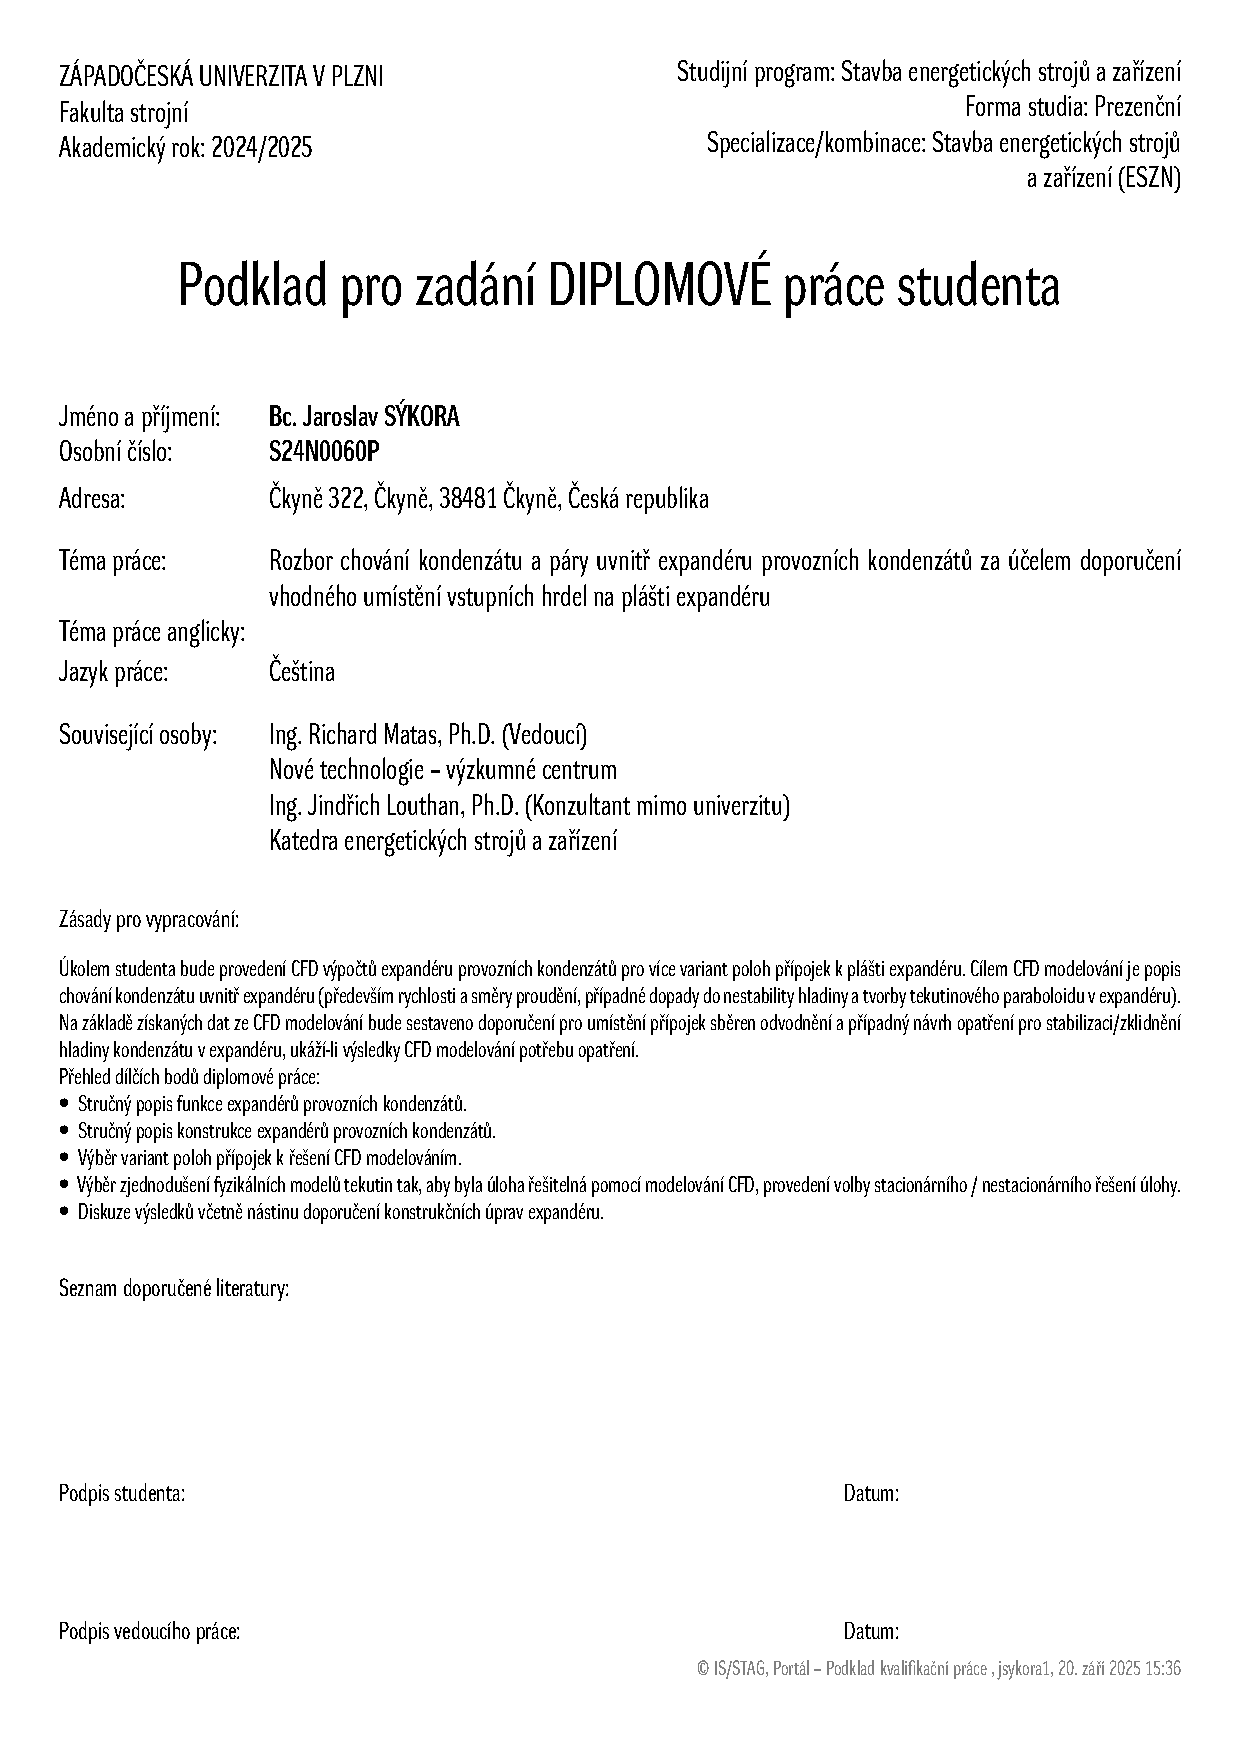
\includepdf[pages=-]{zadani.pdf}	% pages=- importuje všechny stránky


% anotační list CZ
{
\newcolumntype{Y}{>{\centering\let\newline\arraybackslash\hspace{0pt}}X}	
\newcolumntype{C}[1]{>{\centering\let\newline\\\arraybackslash\hspace{0pt}}m{#1}}
\newcolumntype{E}{>{\centering\let\newline\\\arraybackslash\hspace{0pt}}m{9.4cm}}
\def\Z{\vphantom{\parbox[c][1.2cm]{0.5cm}{}}}	

\clearpage
\pdfbookmark[2]{Anotační list}{anotace}		
\begin{center}\MakeUppercase{\Large\bfseries{Anotační list bakalářské práce}}\end{center} 	
\vspace{1cm}
\noindent\begin{tabularx}{\textwidth}{| Y | C{4.5cm} | C{4.5cm} |}
	\hline
	\Z \Nad{Autor} & \FilN{Příjmení}{\Aprijmeni,\,\Atituly} & \FilN{Jméno}{\Ajmeno} \\ \hline
	\Z \Nad{Studijní obor} & \multicolumn{2}{E|}{\programN--\oborCZ}  \\ \hline
	\Z \Nad{Vedoucí práce} & \FilN{Příjmení}{\Vprijmeni,\,\VtitulyP,\,\VtitulyZ} & \FilN{Jméno}{\Vjmeno} \\ \hline
	\Z \Nad{Pracoviště} & \multicolumn{2}{E|}{\pracovisteCZ}  \\ \hline
	\Z \Nad{Druh práce} & \Nad{Diplomová} & \sout{\Nad{Bakalářská}} \\ \hline 
	\Z \Nad{Studijní obor} & \multicolumn{2}{E|}{\nazevCZ}  \\ \hline
\end{tabularx}
	
\vspace{1cm}
\noindent\begin{tabularx}{\textwidth}{|@{}Y@{}|C{2.2cm}||@{}Y@{}|C{1cm}||@{}Y@{}|C{1cm}|}
	\hline
	\Z \Nad{Fakulta} & \fakultaCZ & \Nad{Katedra} & \ZkatedraCZ &  \parbox[c]{3cm}{\centering\Nad{Rok odevzdání}} & \Rokodevzdani \\ \hline
\end{tabularx}

\vspace{1cm}
\noindent{\textbf{Počet stran (A4 a ekvivalentů A4)}}

\noindent\begin{tabularx}{\textwidth}{|@{}Y@{}|C{2.2cm}||@{}Y@{}|C{1cm}||@{}Y@{}|C{1cm}|}
	\hline
	\Z \Nad{Celkem} & \Pcelkem &\parbox[c]{3cm}{\centering\Nad{Textová část}} & \Ptext &  \parbox[c]{3cm}{\centering\Nad{Grafická část}} & \Pgraphic \\ \hline
\end{tabularx}

\vspace{1cm}
\noindent\begin{tabularx}{\textwidth}{| Y |m{10cm} |}
	\hline
	\Z \Nad{Stručný popis} & \abstrCZ \\ \hline
	\Z \Nad{Klíčová slova} & \klicovaCZ \\ \hline
\end{tabularx}

\newpage
	
\begin{center}\MakeUppercase{\Large\bfseries{Summary of BACHELOR sheet\phantom{ř}}}\end{center} 
\vspace{1cm}
\noindent\begin{tabularx}{\textwidth}{| Y | C{4.5cm} | C{4.5cm} |}
	\hline
	\Z \Nad{Author} & \FilN{Surname}{\Aprijmeni,\,\Atituly} & \FilN{Name}{\Ajmeno} \\ \hline
	\Z \parbox[c]{3cm}{\centering\Nad{Study \mbox{programme}}} & \multicolumn{2}{E|}{\programN--\oborEN}  \\ \hline
	\Z \Nad{Supervisor} & \FilN{Surname}{\Vprijmeni,\,\VtitulyP,\,\VtitulyZ} & \FilN{Name}{\Vjmeno} \\ \hline
	\Z \Nad{Institution} & \multicolumn{2}{E|}{\pracovisteCZ}  \\ \hline
	\Z \Nad{Type of work} & \Nad{Diploma} & \sout{\Nad{Bachelor}} \\ \hline 
	\Z \parbox[c]{3cm}{\centering\Nad{Title of the work}} & \multicolumn{2}{E|}{\nazevEN}  \\ \hline
\end{tabularx}

\vspace{1cm}
\noindent\begin{tabularx}{\textwidth}{|@{}Y@{}|C{2.2cm}||@{}Y@{}|C{1cm}||@{}Y@{}|C{1cm}|}
	\hline
	\Z \Nad{Faculty} & \fakultaEN &\parbox[c]{3cm}{\centering\Nad{Depart\-ment}} & \ZkatedraCZ &  \parbox[c]{3cm}{\centering\Nad{Submitted in}} & \Rokodevzdani \\ \hline
\end{tabularx}

\vspace{1cm}
\noindent{\textbf{Number of pages (A4 and equivalent of A4)}}

\noindent\begin{tabularx}{\textwidth}{|@{}Y@{}|C{2.2cm}||@{}Y@{}|C{1cm}||@{}Y@{}|C{1cm}|}
	\hline
	\Z \Nad{Totally} & \Pcelkem &\parbox[c]{2cm}{\centering\Nad{Text part}} & \Ptext &  \parbox[c]{3cm}{\centering\Nad{Graphical part}} & \Pgraphic \\ \hline
\end{tabularx}

\vspace{1cm}
\noindent\begin{tabularx}{\textwidth}{| Y |m{10cm} |}
	\hline
	\Z \parbox[c]{4cm}{\centering\Nad{Brief description}} & \abstrEN \\ \hline   % Stručný popis   Brief description
	\Z \Nad{Key words} & \klicovaEN \\ \hline
\end{tabularx}
}
	\clearpage
	\pdfbookmark[1]{Obsah}{loc}		
	\tableofcontents		% obsah
	
	\clearpage
	\pdfbookmark[2]{Seznam obrázků}{lof}		
	\listoffigures			% seznam obrázků
	
	\clearpage
	\pdfbookmark[2]{Seznam tabulek}{lot}		
	\listoftables			% seznam tabulek
	
	% \clearpage
	% \pdfbookmark[2]{Seznam algoritmů}{lol}		
	% \lstlistoflistings		% sezam kódů
	
	\thispagestyle{empty}	% Odstraní číslování z poslední strany

}

{
\pagestyle{empty}

% seznam zkratek  
\clearpage
\pdfbookmark[2]{Seznam veličin a indexů}{listofquantity}
\chapter*{Seznam veličin a indexů}
\thispagestyle{empty}
\renewcommand{\arraystretch}{1.1}	% větší mezery mezi zkratkami nikoliv mezi řádky
\begin{xltabular}{\linewidth}{@{}l X r@{}}
	\tb{Veličina} & \tb{Popis} & \tb{Rozměr}\\\hline
	\rule{2cm}{0pt}& &\rule{2cm}{0pt} \\\endhead
	% seznam použitých jednotek
% nutno řadit ručně abecdně, script není
% formát: $m_{cel}$ & celkový hmotnostní průtok & {[}\si{\kilogram\per\second}{]} \\
$m$ & Hmotnost & {[}\si{\kilogram}{]} \\

 %indexi
\tb{Index}\\ \hline
\\
$max$ & Maximální hodnota\\


\end{xltabular}
\thispagestyle{empty}
}

% seznam veličin
{
	\pagestyle{empty}
	\clearpage
	\pdfbookmark[2]{Seznam zkratek}{listofabb}
	\chapter*{Seznam zkratek}
	\thispagestyle{empty}
	\renewcommand{\arraystretch}{1.2}	% větší mezery mezi zkratkami nikoliv mezi řádky
	\begin{xltabular}{\linewidth}{@{}>{\bfseries}l X@{}}
		\tb{Zkratka} & \tb{Význam}\\\hline 
		\rule{2cm}{0pt}&\\\endhead
		% seznam zkratek
% nutno řadit ručně abecdně, script není
% forát: zkratka & význam zkratky
% & \\

ISO     & \foreignlanguage{english}{International Organization for Standardization} -- Mezinárodní organizace pro normalizaci \\
ČSN     & \foreignlanguage{english}{Czech technical standard} -- Česká technická norma\\
FFT     & \foreignlanguage{english}{Fast Fourier transform} -- Rychlá Fourierova transformace\\
CFD    & \foreignlanguage{english}{Computational fluid dynamics} -- Výpočetní dynamika tekutin\\
CAA    & \foreignlanguage{english}{Computational Aeroacoustic} -- Výpočetní aeroakustika\\	
\end{xltabular}
\thispagestyle{empty}
}

\pagestyle{fancy}

% Úvod
\chapter*{Úvod}\label{chap:uvod}
\addcontentsline{toc}{chapter}{Úvod}

Při prodeji, respektive nabízení turbíny, je potřeba garantovat zákazníkovi parametry tohoto zařízení. Tyto parametry se zpravidla liší a je na zákazníkovi, jak přísné požadavky bude mít. Například může jít o výkon turbíny, její účinnost, životnost, odolnost vůči zemětřesení a tak dále. 

Stále častěji je na výrobce turbín kladen nárok ohledně garance maximální hladiny akustického tlaku, kterou zařízení při provozu nesmí překročit. Hlavní důvod takového požadavku je ochrana zdraví pracovníků, kteří pracují v blízkosti zařízení. Takový požadavek vznášejí převážně vyspělé země, ve kterých je ochrana pracovníka na prvním místě. Schopnost garantovat maximální zvuk turbíny tedy může znamenat konkurenční výhodu.

Práce se bude nejprve zabývat fyzikální podstatou zvuku a odvozením základních vztahů. Následně budou popsány nesrovnalosti při porovnávání naměřených dat s vnímáním zvuku lidským organismem. S tím souvisí používaní filtrů, které problematiku berou v potaz.

Při analýze turbíny za provozu odhalila společnost Doosan Škoda Power několik zdrojů zvuku. Způsob měření je normalizován a popis tohoto měření je uveden níže v práci. Vyhodnocení dat ukázalo, že nejvýznamnějším zdrojem je rotující spojka mezi turbínou a generátorem. Proto se bakalářská práce zabývá právě touto spojkou.

Po obvodu a na čele spojky se nachází několik otvorů, které by mohly zvuk způsobovat. Závitové díry po obvodu slouží pro našroubování vývažků, válcové díry slouží pro pojištění šroubů proti povolení a díry na čele spojky slouží pro sešroubování dvou kotoučů spojky. Součástí práce bude také popsat, jak geometrie a umístění těchto děr ovlivňuje frekvenci a intenzitu zvuku. 

Tento problém lze řešit dvěma způsoby. Jako první řešení lze použít zvukopohltivé kryty, ty jsou ale drahé a nemají jistý výsledek. Druhou možností jsou záslepky pískajících otvorů. Ty jsou spolehlivější, ovšem jejich přidáním může vzniknout nevývažek. Proto je snaha pochopit přímou příčinu vzniku akustického tlaku. Na základě těchto poznatků je potřeba navrhnout takové řešení, aby k problému nedocházelo.

Pro správné pochopení problému je nutné nejdříve popsat fyzikální význam akustického tlaku. Přesněji to, jak se šíří, jakými způsoby ho můžeme měřit a také to, jak na problematiku pohlíží normy.  







% Závěr
\chapter*{Závěr}
\addcontentsline{toc}{chapter}{Závěr}

První část práce se zabývala definováním všech akustických veličin, které jsou dále v práci používány, například rychlostí zvuku v prostředí, frekvencí zvuku a tak dále. Byly zde popsány základní principy šíření zvuku v prostředí. Dalším důležitým bodem teoretické části práce byl popis akustických hladin a práce s logaritmickou škálou. v závěru teoretické části byla popsána frekvenční pásma použitá při vyhodnocování naměřených dat.
\par I přesto, že se práce zaměřuje na technické řešení problému, bylo nutné také popsat, jak lidské tělo reaguje na zvuk a proč je nutné dbát na hlučnost prostředí, ve kterém lidé pracují. 
\par Zásadní byl popis měřidel, která byla použita při experimentech. Při zkoumání problematiky provedla společnost Doosan Škoda Power hned několik experimentů, v práci jsou tedy zdůvodněny použité metody měření a stručně popsány varianty měření. Zobrazené jsou také výsledky měření z prvních třech variant, tyto výsledky byly zpracovány prostřednictvím Matlab scriptu.
\par Výsledky měření byly srovnány s výsledky získanými analytickou metodou. Tato metoda je vhodná pro předpovídání frekvenčních špiček pro daný otvor. Nelze však předpovídat velikost akustické hladiny vzniklého zvuku. Pro hlubší pochopení problému by bylo nejspíše nutné provést CFD a CAA simulace opřené o experiment.
\par Nakonec práce byla navržena konstrukční úprava spojky, která by měla snížit hlučnost. Tato úprava však zatím není v praxi použita, jelikož výsledek tohoto řešení není jistý a v případě nedostatečného útlumu by nebylo možné použít zaslepení děr \cite{bartel_possible_2021}. 

	% vlastní práce
\printbibheading[title=Literatura]
\pdfbookmark[1]{Knihy}{knihy}
\printbibliography[heading=subbibliography,type=book,title={Knihy}]	
%\addcontentsline{toc}{section}{Knihy}

\pdfbookmark[1]{Články}{clanky}
\printbibliography[heading=subbibliography,type=article,title={Články}]	
%\addcontentsline{toc}{section}{Články}


\pdfbookmark[1]{Online}{online}
\printbibliography[heading=subbibliography,filter=zbytek,title={Online}]
%\addcontentsline{toc}{section}{Online}	


\appendix
\renewcommand{\thechapter}{\arabic{chapter}}
\addtocontents{toc}{\protect\vskip50pt}
%\chapter{Měřený kotouč}
\chapter{Space Holder}


\end{document}
